% !Mode:: "TeX:UTF-8"

\chapter{Servlet 项目}

\section{项目需求}

本项目要求使用VUE+Servlet+AJAX技术,开发前后端分离的饿了么Web应用程序。主要设计参照 “饿了么官网网页版”制作,并且仅关注点餐业务线功能,“饿了么官网”中的其它功能暂不涉及。

本项目需要完成的功能大致分为十一个页面:

1.首页:显示点餐分类信息

2. 商家列表页面:根据点餐分类显示商家列表信
息, 如果处于登录状态,那些需要
查询购物车中是否有此商家的
食品。如果有,在页面上显示
食品数量。

3.商家详细信息页面:显示商家详细信息及所属食品信
息,并自动计算总价。

4.确认订单页面:确认订单信息是否正确;选择送货地址。

5.在线支付页面:显示订单信息及订单明细信息。

6.送货地址页面:显示当前用户的送货地址信息。

7.新增送货地址页面:添加新的送货地址。

8.编辑送货地址页面:编辑送货地址。

9.登录页面:用户登录。

10.注册页面:注册新用户。

11.历史订单页面:显示用户历史订单信息。~\\


\section{项目设计}

1.数据库设计:

本项目使用MySQL数据库,选择DataGrip作为开发工具。在数据表的设计上,需要创建商家表、食品表、购物车表、送货地址表、订单表、订单明细表、用户表共七张表。
\begin{figure}[H]
    \centering
    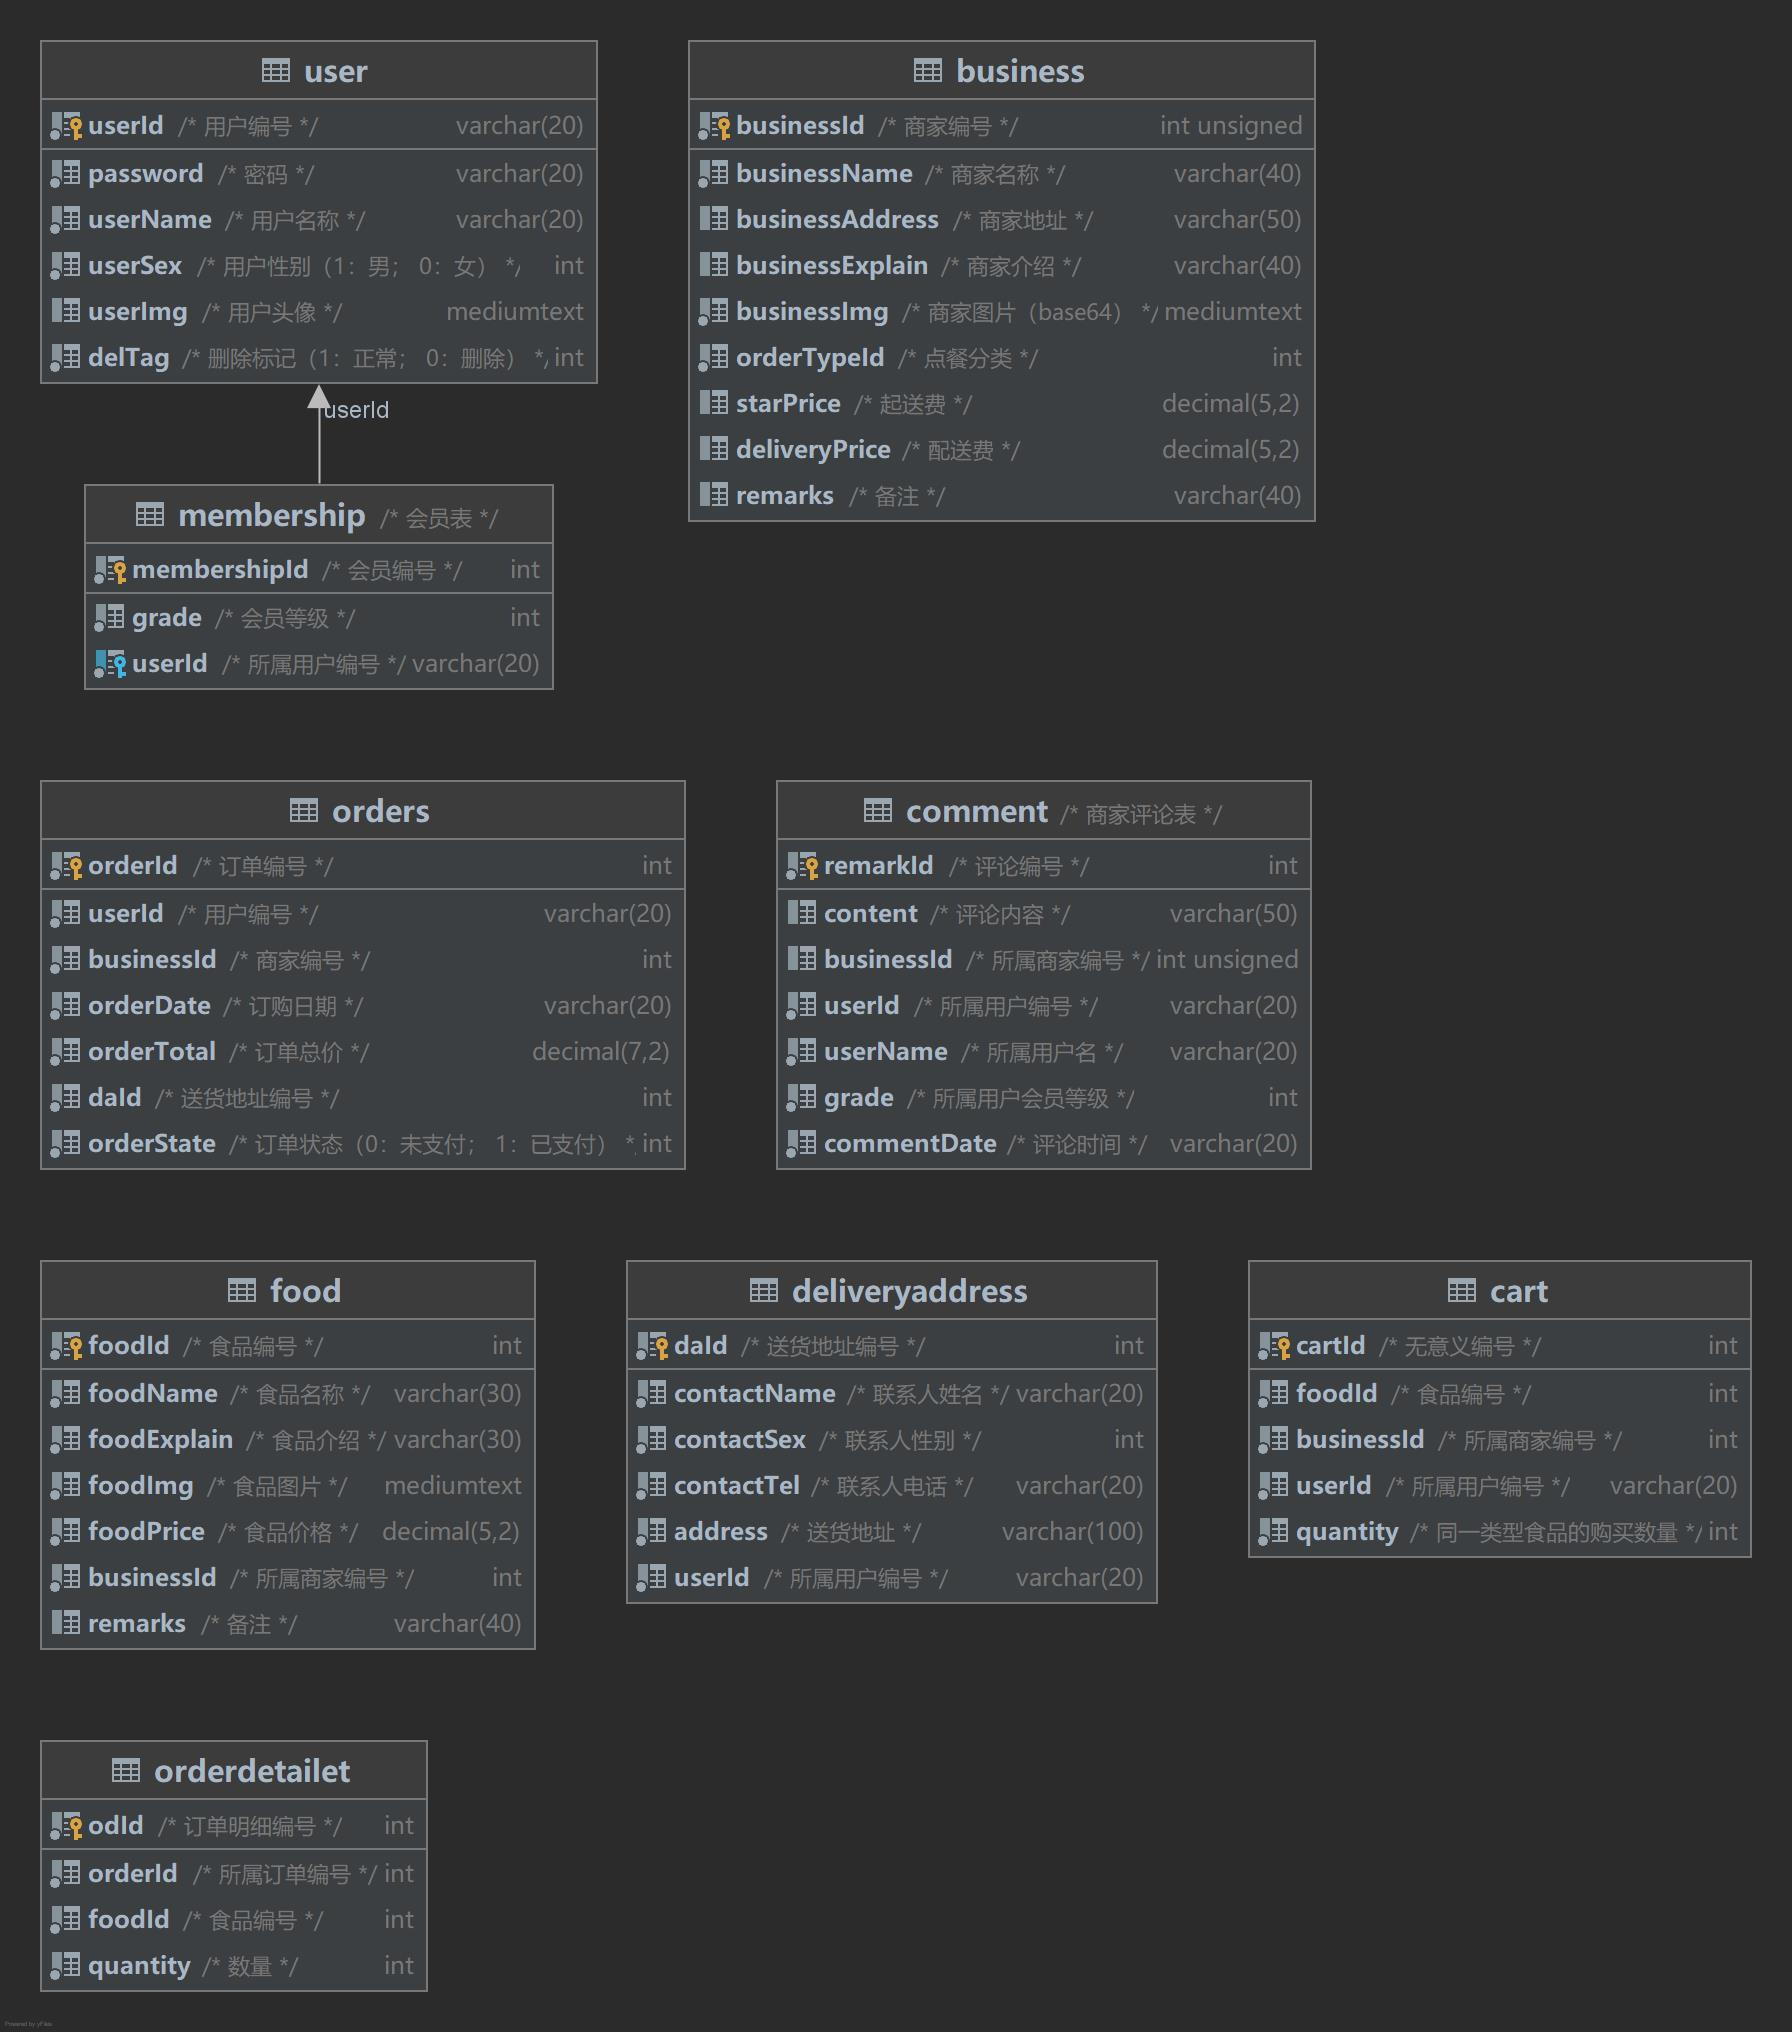
\includegraphics[width=15cm,height=17cm]{figures/table2.jpg}
    \caption{Servlet项目数据表}
    \end{figure}

2.服务器端设计:



